\newpage
\chapter{Theoretical background}
\newpage

\section{Business Model}

\section{Chatbot}
\subsection{Overview of chatbot}

%https://botscrew.com/blog/what-are-bots/

Chatbot is a computer program that simulates a natural human conversation. Users communicate with a chatbot via the chat interface or by voice, like how they would talk to a real person.

Chatbots interpret and process user’s words or phrases and give an instant pre-set answer. They inhabit platforms like – FB Messenger, Whatsapp, Skype, Slack, Line, Kik, Wechat or even your website.  Similar to regular apps chatbots have application layer, a database, APIs and Conversational User Interface (CUI).

There are three main types of chatbots:
\begin{itemize}
\item Rule-based chatbots
\item Intellectually independent chatbots
\item AI-powered chatbots
\end{itemize}


\subsubsection{Rule-based chatbots}

This is the simplest type of chatbots today. People interact with these bots by clicking on buttons and using pre-defined options. To give relevant answers these chatbots require people to make a few selections. As a result, these bots have longer user journey, and they are the slowest to guide the customer to their goal.

These bots are great when it comes to qualifying your leads. The chatbot – asks questions, and people answer them with buttons. The bot analyzes collected data and gives a reply. But, for more advanced scenarios with many conditions or factors, these chatbots aren’t always the best solution.

\subsubsection{Intellectually independent chatbots}

These bots use Machine Learning (ML) which helps the chatbot learn from user’s inputs and requests.

ML is the ability of the computer to learn by itself from the data, recognize patterns and decide with minimal human interference.

Intellectually independent chatbots are trained to understand specific keywords and phrases that trigger bot’s reply. With the time they train themselves to understand more and more questions. You can say they learn and train from experience.

For example, you write to a chatbot: “I have a problem with logging into my account”. The bot would understand the words “problem” “logging” “account” and would provide a pre-defined answer based on these phrases.

\subsubsection{AI-powered chatbots}

AI-powered bots combine the best from Rule-based and Intellectually independent.

Artificial Intelligence (AI) is a simulation of human intelligence. AI is the area of computer science that focuses on creating intelligent machines that work and “think” as people.

AI-powered chatbots understand free language, but also have a predefined flow to make sure they solve user’s problem. They can remember the context of the conversation and the user’s preferences. These chatbots can jump from one point of conversation scenario to another when needed and address random user request at any moment.

These chatbots use Machine Learning, AI and Natural Language Processing (NLP) to understand people.

NLP is the ability of the computer to understand and analyze human speech, find the right response and reply in understandable for a human language.

The goal of NLP is to make the interaction between computers and humans feel like communication between two people. With the help of NLP people can freely interact with chatbots asking a question.

\subsubsection{Chatbot in this project}

We plan to build a AI-powered chatbot application as a virtual assistant, friendly, convenient and can collect a lot of user information to make recommendations about products they may like from the service Providers. In this system, chatbot will have to meet the following criteria:
\begin{itemize}
\item Through NLU understand user intent and requirements.
\item Serve daily conversations as a virtual assistant, meet certain needs of users and collect user information.
\item From the collected conversations, information as well as user preferences.
\item Use collected information to suggest appropriate products and services.
\item Give suggestions and help users get in touch with the supplier of products and services quickly.
\end{itemize}

\subsection{How does chatbot work?}

There are many different ways to build a chatbot, but the most effective way currently is to use natural language processing (NLP).
Chatbots use NLP to finds a way to convert the user’s speech or text into structured data. Which is then utilized to choose a relevant answer. Natural Language Processing includes the following steps;


\begin{itemize}
\item Tokenization: The NLP separates a series of words into tokens or pieces that are linguistically representative, with a different value in the application.
\item Sentiment Analysis: It will study and learn the user’s experience, and transfer the inquiry to a human when necessary
\item Normalization: This program model processes the text to find out the typographical errors and common spelling mistakes that might alter the intended meaning of the user’s request.
\item Named Entity Recognition: The program model of chatbot looks for different categories of words, similar to the name of the particular product, the user’s address or name, whichever information is required.
\item Dependency Parsing: The Chatbot searches for the subjects, verbs, objects, common phrases and nouns in the user’s text to discover related phrases that what users want to convey.
\end{itemize}

\subsubsection{Intent classification}

Intent classification is an automatic classification of a user's input into specified intentions. For example, with the input "I want to buy apples", the chatbot can indicate the user's intention to "buy fruit".

In a technical view, intent classification can be considered similar to document classification on short documents, so one of the simplest ways to make an intent classification is to use the tf-idf matrix.

\subsubsection{Entities recognition}

Chatbots can use intent classification to understand user intent. However, in some cases, the intention is not enough to serve the user. For example, with the saying "I want to buy apples", the chatbot can understand the intent of "buying fruits", but still can't know what kind of fruit it is, we can't use hundreds of other intents as well. for hundreds of fruits, this is the reason entity recognition is needed.

Entities recognition is automatically finding entities in sentences and classifying them. For example, with the phrase "I want to buy apples", chatbots need to indicate that "apple" is an entity "fruit" in the sentence. Then, with the above statement, chatbots can understand it with the form \{intent: "buy fruit", entities: \{"fruit": "apples"\}\}

There are many libraries available for entities recognition such as Standford NER, Spacy, Nltk, etc. they provide a list of common entities, however, to use custom entities, chatbots need data for those entities and train them with their own models or libraries.

\subsection{Rasa}
\subsubsection{What is Rasa}

Rasa Open Source is a conversational AI framework for building contextual assistants.
Rasa Open Source includes

\begin{itemize}
\item NLU: determines what the user wants and captures key contextual information
\item Core: selects the next best response or action based on conversation history
\item Channels and integrations: connect assistant to users and backend systems
\end{itemize}

\subsubsection{Rasa NLU}

Rasa NLU is an open-source natural language processing tool for intent classification, response retrieval and entity extraction in chatbots. For example, taking a sentence like.

\textit{"I am looking for a Mexican restaurant in the center of town"}

and returning structured data like

\{

  \quad"intent": "search\_restaurant",
  
  \quad"entities": \{
  
    \qquad"cuisine" : "Mexican",
    
    \qquad"location" : "center"
    
  \quad\}
  
\}

\subsubsubsection{NLU components}
Rasa NLU uses different NLU components, each with different functions and algorithms. Here are some common components in Table \ref{tab:rasacomponent}

\begin{table}
\caption{Rasa NLU components}
\centering
\begin{tabular}{p{5cm}|p{4cm}|p{8cm}}
Name                                                                   & Function              & Description                                                                                                              \\ 
\hline
SpacyNLP                                                               & Word vector extractor & SpaCy language initializer                                                                                               \\
SpacyFeaturizer                                                        & Text Featurizer       & SpaCy intent featurizer                                                                                                  \\
RegexFeaturizer                                                        & Text Featurizer       & Regex feature creation to support intent and entity classification                                                       \\
CountVectorsFeaturizer                                                 & Text Featurizer       & Creates bag-of-words representation of user message and label (intent and response) features                             \\
SklearnIntentClassifier                                                & Intent Classifier     & Sklearn intent classifier                                                                                                \\
EmbeddingIntentClassifier                                              & Intent Classifier    & Embedding intent classifier                                                                                              \\
WhitespaceTokenizer                                                    & Tokenizer             & Tokenizer using whitespaces as a separator                                                                               \\
SpacyTokenizer                                                         & Tokenizer             & Tokenizer using spacy                                                                                                    \\
SpacyEntityExtractor                                                   & Entity Extractor      & SpaCy entity extraction                                                                                                  \\
EntitySynonymMapper                                        & Entity Extractor      & Maps synonymous entity values to the same value.                                                                         \\
CRFEntityExtractor                                                     & Entity Extractor      & Conditional random field entity extraction                                                                               \\
DucklingHTTPExtractor                                                  & Entity Extractor      & Duckling lets you extract common entities like dates, amounts of money, distances, and others in a number of languages. 
\end{tabular}
\label{tab:rasacomponent}
\end{table}

\subsubsubsection{NLU pipeline}

NLU pipeline is built from NLU components, forming a pipeline of components, from here, user input will go through each component until the final ouput is released.
The NLU pipeline can be customized, replaced, and changed in order of components to get the best results depending on the purpose of using the chatbot.
Here is an example of NLU pipeline configuration:

\quad pipeline:

\qquad - name: "SpacyNLP"

\qquad - name: "SpacyTokenizer"

\qquad - name: "SpacyFeaturizer"

\qquad - name: "RegexFeaturizer"

\qquad - name: "CRFEntityExtractor"

\qquad - name: "EntitySynonymMapper"

\qquad - name: "SklearnIntentClassifier" 

Once the pipeline is defined, each component is called one after another and produces the output which is either directly added to the Rasa NLU model output, or used as an input for other components. For example,  three components in pipeline ["Component1", "Component2", "Component3"], the methods of the "Component1" will be called first. An image 2.1 below shows the component lifecycle:

\begin{figure}[h]
    \label{fig:rasacomponentlifecycle}
    \centering
    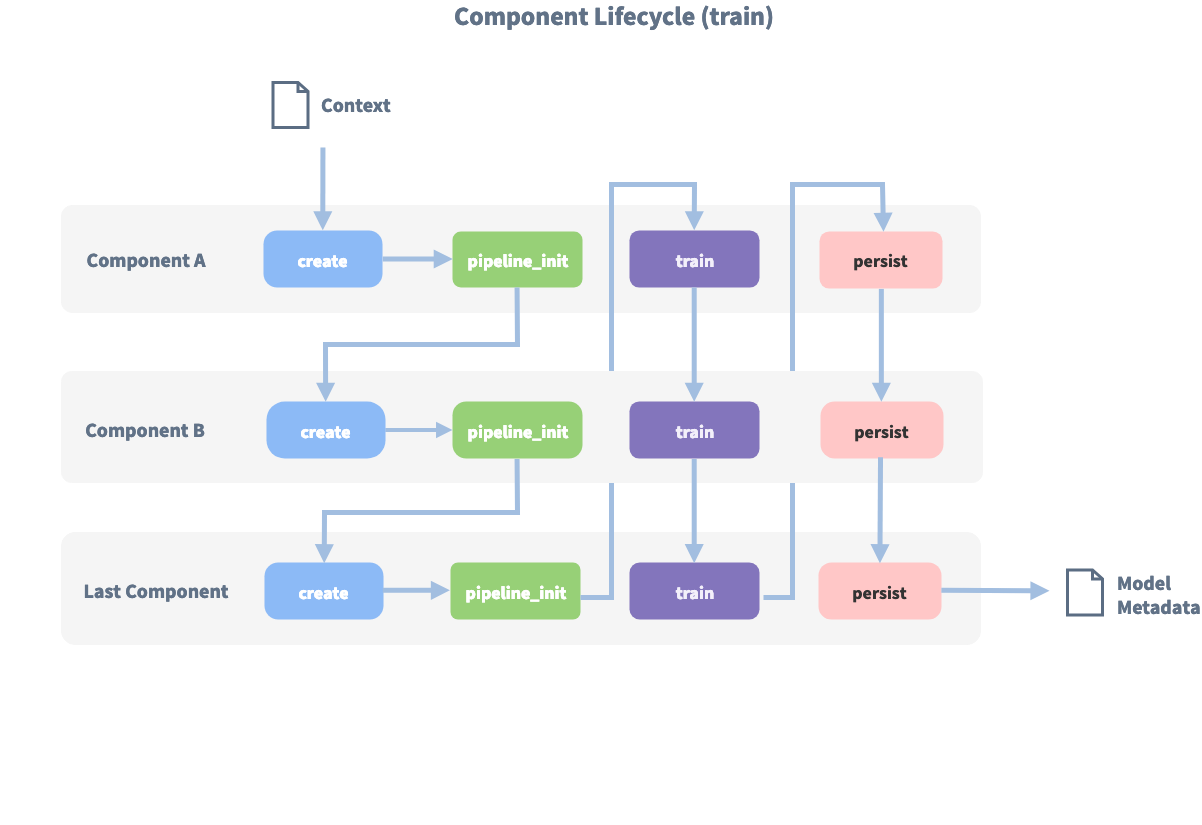
\includegraphics[width=1\textwidth]{Picture/Rasa-Component-Lifecycle--Train-.png}
    \caption{Rasa component lifecycle}
\end{figure}

Components go through the three main stages:
\begin{itemize}
\item Create: initialization of the component before the training
\item Train: the component trains itself using the context and potentially the output of the previous components
\item Persist: saving the trained component on disk for the future use
\end{itemize}
Before the first component is initialized, a so-called context is created which is used to pass the information between the components. For example, one component can calculate feature vectors for the training data, store that within the context and another component can retrieve these feature vectors from the context and do intent classification. Once all components are created, trained and persisted, the model metadata is created which describes the overall NLU model.

\subsubsection{Rasa core}

While Rasa NLU is a library for extracting information from user input into a data structure that chatbots can understand, Rasa core is used to build a system that can use those data. extracted from Rasa NLU and processed information, provided response and manipulated chatbot's conversation.

\subsubsubsection{Intent}

Intent is the intent in the user's statement, the intent information provided by the NLU model includes their entire intent and confidence list, Rasa core will usually choose the intent with the highest confidence to understand that the user intent in saying.
An example intent is returned to the Rasa core:

\{

    \quad"intent": {"name": "greet", "confidence": 0.8343},

    \quad"intent\_ranking": [

        \qquad\{

            \qquad\quad"confidence": 0.385910906220309,

            \qquad\quad"name": "goodbye"

        \qquad\},

        \qquad\{

            \qquad\quad"confidence": 0.28161531595656784,

            \qquad\quad"name": "restaurant\_search"

        \quad\}

    ]

\}

In Rasa, intent is extracted by Intent Classifier components. Rasa reads the intent from the training sets as markdown or json.

\textbf{Markdown Format}

Markdown is the easiest Rasa NLU format for humans to read and write. Examples are listed using the unordered list syntax, e.g. minus -, asterisk *, or plus +. Examples are grouped by intent, and entities are annotated as Markdown links, e.g. [entity](entity name).

\begin{figure}[h]
    \label{fig:markdownexample}
    \centering
    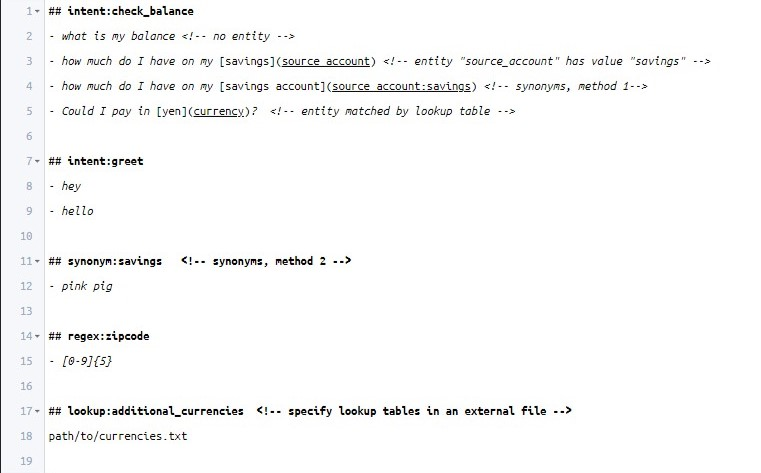
\includegraphics[width=1\textwidth]{Picture/markdownexample.jpg}
    \caption{Markdown training format example}
\end{figure}

\textbf{JSON Format}

The JSON format consists of a top-level object called \textit{rasa\_nlu\_data}, with the keys\textit{ common\_examples},\textit{ entity\_synonyms} and \textit{regex\_features}. The most important one is \textit{common\_examples}.
\newline
\newline

\{

    \qquad"rasa\_nlu\_data": \{

        \qquad"common\_examples": [ ],

        \qquad"regex\_features" : [ ],

        \qquad"lookup\_tables"  : [ ],

        \qquad"entity\_synonyms": [ ]

    \quad\}

\}

The \textit{common\_examples} are used to train your model. You should put all of your training examples in the \textit{common\_examples} array. Regex features are a tool to help the classifier detect entities or intents and improve the performance.

\subsubsubsection{Entity}

Rasa uses Entity Extractor components to extract entities from user input, below is an example of entities returned to Rasa core.
\\*

\{

  \quad"text": "show me chinese restaurants",

  \quad"intent": "restaurant\_search",

  \quad"entities": [

    \qquad\{

      \quad\qquad"start": 8,

      \quad\qquad"end": 15,

      \quad\qquad"value": "chinese",

      \quad\qquad"entity": "cuisine",

      \quad\qquad"extractor": "CRFEntityExtractor",

      \quad\qquad"confidence": 0.854,

      \quad\qquad"processors": []

    \qquad\}

  \quad]

\}
\\*

Some extractors, like \textit{duckling}, may include additional information. For example:
\\*

\{
  
  \quad"additional\_info":\{

    \qquad"grain":"day",

    \qquad"type":"value",

    \qquad"value":"2018-06-21T00:00:00.000-07:00",

    \qquad"values":[

      \quad\qquad\{

        \qquad\qquad"grain":"day",

        \qquad\qquad"type":"value",

        \qquad\qquad"value":"2018-06-21T00:00:00.000-07:00"

      \quad\qquad\}

    \qquad]

  \quad\},

  \quad"confidence":1.0,

  \quad"end":5,

  \quad"entity":"time",

  \quad"extractor":"DucklingHTTPExtractor",

  \quad"start":0,

  \quad"text":"today",

  \quad"value":"2018-06-21T00:00:00.000-07:00"

\}
\\*

Training for Entities can also be written as markdown or json (example from \ref{fig:markdownexample}).

\subsubsubsection{Slot}

Slots are chatbot’s memory. They act as a key-value store which can be used to store information the user provided (e.g their home city) as well as information gathered about the outside world (e.g. the result of a database query).

Slots to influence how the dialogue progresses. There are different slot types for different behaviors.

For example, if user has provided their home city, you might have a text slot called home\_city. If the user asks for the weather, and you don’t know their home city, you will have to ask them for it. A text slot only tells Rasa Core whether the slot has a value. The specific value of a text slot (e.g. Bangalore or New York or Hong Kong) doesn’t make any difference.

If the value itself is important, use a categorical or a bool slot. There are also float, and list slots. Unfeaturized slot can be used to store data which is not important to the conversation.

\subsubsubsection{Story}

Rasa stories are a form of training data used to train the Rasa’s dialogue management models.

A story is a representation of a conversation between a user and an AI assistant, converted into a specific format where user inputs are expressed as corresponding intents (and entities where necessary) while the responses of an assistant are expressed as corresponding action names.

Here’s an example of a dialogue in the Rasa story format:

\begin{figure}[h]
    \label{fig:storyexample}
    \centering
    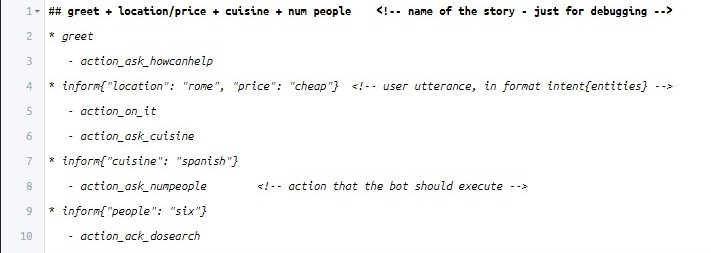
\includegraphics[width=1\textwidth]{Picture/storyexample.jpg}
    \caption{Story training format example}
\end{figure}

Story will tell chatbot what to do after each user action. Each action is a pre-implemented function of the Rasa core, after each intent, the Rasa core will determine the next action based on what has been trained from the story.
Usually, the Rasa core will find a story that exactly matches the conversation first, then take the next action based on that. If no stories are found, the Rasa core will make predictions through the model trained on the stories, which makes our chatbot adapt to completely new conversations.

\subsubsubsection{Action}

Actions are the things chatbot runs in response to user input. There are four kinds of actions in Rasa:


\begin{itemize}
\item Utterance actions: start with utter\_ and send a specific message to the user
\item Retrieval actions: start with respond\_ and send a message selected by a retrieval model
\item Custom actions: run arbitrary code and send any number of messages (or none).
\item Default actions: e.g. action\_listen, action\_restart, action\_default\_fallback
\end{itemize}

Utterance action is simply a message returned from chatbot, it can be a form or a list of choices, etc. However, the utterance action cannot handle complex actions such as retrieving data from a database or processing complex processes.

To handle complex tasks, we use custom actions, which need to be implemented from scratch. Rasa core provides a separate library for building custom actions, but we can implement another library for custom actions because these actions operate on a server independent of Rasa core.

\section{Recommender System}

\subsection{What is recommender system?}
A recommender system is a subclass of information filtering system that seeks to predict the "rating" or "preference" a user would give to an item. They are primarily used in commercial applications. recommender systems are utilized in a variety of areas, and are most commonly recognized as playlist generators for video and music services like Netflix, YouTube and Spotify, product recommendations for services such as Amazon, or content recommenders for social media platforms such as Facebook and Twitter.These systems can operate using a single input, like music, or multiple inputs within and across platforms like news, books, and search queries. There are also popular recommender systems for specific topics like restaurants and online dating. Recommender systems have been developed to explore research articles and experts, collaborators, financial services, and life insurance.
\subsection{Collaborative Recommender System}
It’s the most sort after, most widely implemented and most mature technologies that is available in the market. Collaborative recommender systems aggregate ratings or recommendations of objects, recognize commonalities between the users on the basis of their ratings, and generate new recommendations based on inter-user comparisons. The greatest strength of collaborative techniques is that they are completely independent of any machine-readable representation of the objects being recommended and work well for complex objects where variations in taste are responsible for much of the variation in preferences. Collaborative filtering is based on the assumption that people who agreed in the past will agree in the future and that they will like similar kind of objects as they liked in the past.
\subsection{Content based Recommender System}
It’s mainly classified as an outgrowth and continuation of information filtering research. In this system, the objects are mainly defined by their associated features. A content-based recommender learns a profile of the new user’s interests based on the features present, in objects the user has rated. It’s basically a keyword specific recommender system here keywords are used to describe the items. Thus, in a content-based recommender system the algorithms used are such that it recommends users similar items that the user has liked in the past or is examining currently.
\subsection{Demographic based Recommender System}
This system aims to categorize the users based on attributes and make recommendations based on demographic classes. Many industries have taken this kind of approach as it’s not that complex and easy to implement. In Demographic-based recommender system the algorithms first need a proper market research in the specified region accompanied with a short survey to gather data for categorization. Demographic techniques form “people-to-people” correlations like collaborative ones, but use different data. The benefit of a demographic approach is that it does not require a history of user ratings like that in collaborative and content based recommender systems.
\subsection{Utility based Recommender System}
Utility based recommender system makes suggestions based on computation of the utility of each object for the user. Of course, the central problem for this type of system is how to create a utility for individual users. In utility based system, every industry will have a different technique for arriving at a user specific utility function and applying it to the objects under consideration. The main advantage of using a utility based recommender system is that it can factor non-product attributes, such as vendor reliability and product availability, into the utility computation. This makes it possible to check real time inventory of the object and display it to the user.
\subsection{Knowledge based Recommender System}
This type of recommender system attempts to suggest objects based on inferences about a user’s needs and preferences. Knowledge based recommendation works on functional knowledge: they have knowledge about how a particular item meets a particular user need, and can therefore reason about the relationship between a need and a possible recommendation.
\subsection{Hybrid Recommender System}
Combining any of the two systems in a manner that suits a particular industry is known as Hybrid Recommender system. This is the most sort after Recommender system that many companies look after, as it combines the strengths of more than two Recommender system and also eliminates any weakness which exist when only one recommender system is used. There are several ways in which the systems can be combined, such as:


\begin{itemize}
\item Weighted Hybrid Recommender: In this system the score of a recommended item is computed from the results of all of the available recommendation techniques present in the system. For example, P-Tango system combines collaborative and content based recommendation systems giving them equal weight in the starting, but gradually adjusting the weighting as predictions about the user ratings are confirmed or disconfirmed.Pazzani’s combination hybrid doesn’t use numeric scores but rather treats the output of each recommender as a set of votes, which are then combined in a consensus scheme.
\item Switching Hybrid Recommender: Switching Hybrid Recommender, switches between the recommendation techniques based on particular criterions. Suppose if we combine the content and collaborative based recommender systems then, the switching hybrid recommender can first deploy content based recommender system and if it doesn’t work then it will deploy collaborative based recommender system.
\item Mixed Hybrid Recommender: Where it’s possible to make a large number of recommendations simultaneously, we should go for Mixed recommender systems. Here recommendations from more than one technique are presented together, so it the user can choose from a wide range of recommendations.  The PTV system, mainly a recommended program to suggest customers for television viewing, developed by Smyth and Cotter is used by the majority of the media and entertainment companies.
\end{itemize}
\subsection{Recommender System in this project}
The chatbot will use the Recommendation system to provide users with the services that suit them best, as well as find potential customers for homes. In other words, the chatbot will act as a link between the user and the service provider based on the data collected from the user.

\newpage
\section{Mobile}
\subsection{Overview}

\subsubsection{Native development}
\par{
    Native development is the process of creating software application that can run on specific platforms or devices.
    Some platforms or devices are Smart TV, XBox, Desktop and the environment that is mostly targeted is mobile devices.

    % Reference here https://gs.statcounter.com/os-market-share/mobile/worldwide
    According to statcounter.com in November 2019, Google's Android and Apple's iOS are holding the most market share of
    mobile operating system, 75.85\% and 22.87\% respectively. So in the future, native mobile application development is mostly about Android and iOS.

    \begin{figure}[!ht]
        \centering
        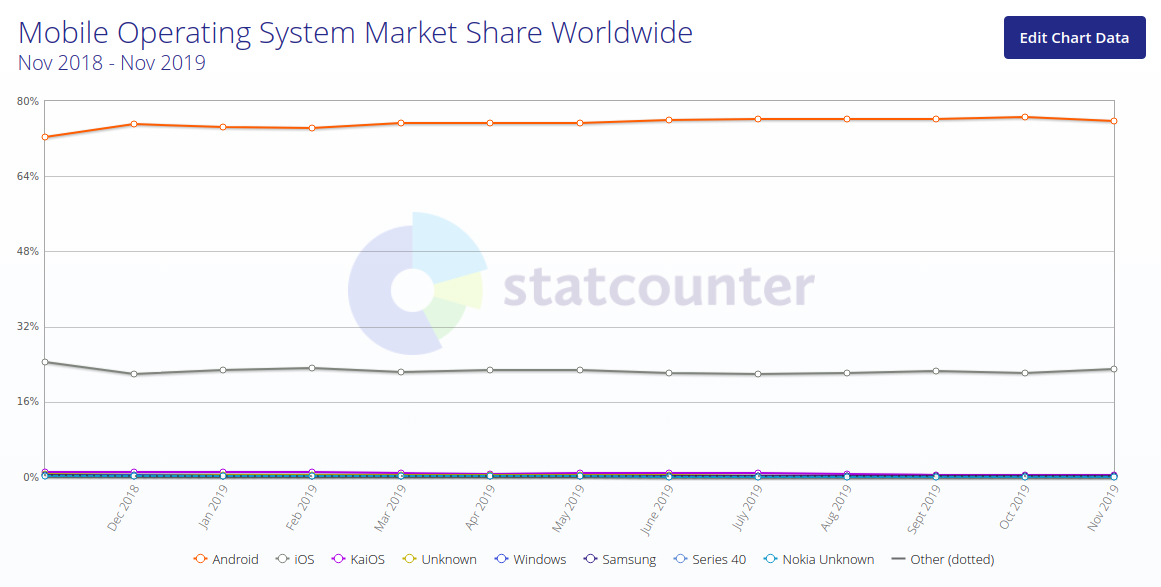
\includegraphics[scale=0.3]{Picture/mobile/mobile_market_share.png}
        \label{fig:logo}
        \caption{Mobile Market Share from Nov 2018 to Nov 2019}
    \end{figure}

    Android supports Java and Kotlin programming languages with various IDEs (Integrated Development Environment), it also has its own IDE - Android Studio for mobile application development.
    On the other hand, iOS requires its native application to be written in Objective C or Swift programming languages using its own IDE - Xcode IDE.

    The platforms have its own high-level APIs (Application Programming Interface) that can be used by developer to implement the UI (User Interface), I/O (Input/Output) operations and other features of their application.
    The result application on each platform will have its own look and feel.
}
\subsubsection{Cross-platform development}
\par{
    The main advantage to cross-platform development over native development is reduce the development team size, time and resources. Another important reason is that the mobile application is an extension to the developer and businesses existing websites. Most companies and start-up reach to more customers by extending their product and service to mobile applications. Airbnb is an example.
    Cross-platform development is mostly preferred by web developers as most cross-platform solutions use web technologies on mobile platforms.
    Cross-platform only uses a single codebase, therefore we only need a single development team for an application that can run on multiple platoforms.
    That is the main reason for cross-platform development.

    Because of the huge difference between platforms such as Android and iOS, and how fast these platforms are growing and developing, creating a cross-platform solution is challenging and nearly impossible task. From various programming languages to different rendering techniques, there are plenty of factors to combine in order to achieve a cross-platform application that can be productive in the long term.
}

\subsubsubsection{Browser-based solutions}
\par{
    Browser-based (or Web-based) mobile application development aims to create cross-platform Web App for any mobile platform using a browser. Some famous technologies out there, Ionic and PhoneGap (previously Apache Cordova), are utilized for this.
    These mobile application are developed using web existing technologies such as HTML (Hypertext Markup Language), CSS (Cascading Style Sheets) and JavaScript running on a WebView of the platform.

    Fast development cycle is what most browser-based approaches have. For instance, Ionic framework provides a live deploy feature that allows developers to directly commit HTML, CSS, and JavaScript updates for bugfixes and future features without the intermediate like App Store. 
    Moreover, the web-like project structure is very convenient to web developers. (See below Figure)
    \begin{figure}[!ht]
        \centering
        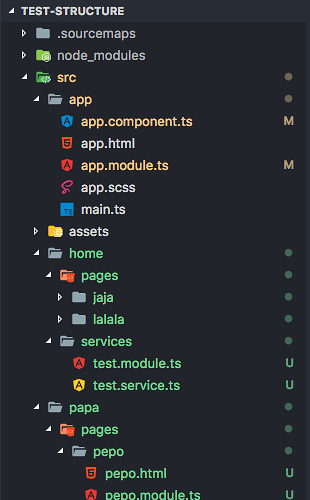
\includegraphics[scale=0.7]{Picture/mobile/ionic_project_structure.png}
        \label{fig:structure_ionic_app}
        \caption{Project structure of Ionic application}
    \end{figure}

    \begin{figure}[!ht]
        \centering
        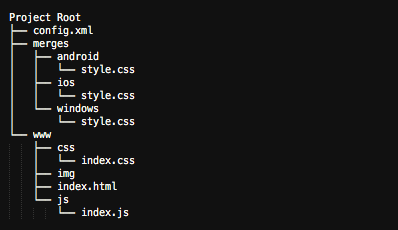
\includegraphics[scale=0.7]{Picture/mobile/phonegap_project_structure.png}
        \label{fig:structure_phonegap_app}
        \caption{Project structure of PhoneGap application}
    \end{figure}
}

\subsubsubsection{Bridging solutions}
\par{
	Bridging approach is an approach that creates a layer above the Native APIs, therefore it will make the software development independent of the platform unlike browser-based approach.
	Facebook's React Native framework is an example for this approach.

	React Native's application is built using JavaScript or TypeScript, but it is not only normal JS or TS, but in React Native, it is JSX or TSX, an extension for the normal JS or TS to embed HTML syntax into JS or TS.
	Underneath that layer, there is a bridge that connected to the native code of the framework.
	Native code of React Native framework container a \textbf{\textit{RootView}} and a \textit{bridge-interface} (For iOs, it is written in Objective C and Java for Android). The \textbf{\textit{RootView}} is the container for all user interface component in the application. The \textit{bridge-interface} serves as an intermediate for the native code of the framework and the bridge.
	
	The heart of React Native, the bridge, forms a bidirectional asynchronous communication
channel between native components inside native frameworks and the JavaScript layer.
This means, when creating an instance of a built-in React Native component (e.g. Text
component), the bridge is responsible for creating the platform specific interface object
(e.g. a subclass of UIView for iOS) with identical/close layout and styling information as
set on the React Native component. User interactions are received in the native
components and propagated to the JavaScript layer via the bridge.
}
\subsubsection{Advantages of cross-platform}
\par{
	Both browser-based approach and bridgin approach allow the mobile application development to have a single codebase, which makes things easier for maintainability. Additionally, the developer can use their web developing experience to apply to create mobile application.

	And some cross-platform approaches do not need the App Store or Google Play's permissions in order to deploy HTML, CSS, and JavaScript updates and bugfixes.
}

\subsubsection{Limitation of cross-platform}
\par{
	Different approaches have their own limitations. Browser-based approach often fails to achieve the feel and look compare to native mobile application because of the difference between web interface components and native components.
	Performance is also a problem in cross-platform mobile development. Because the compilation process involved the convert the code into native components. The more complex the code is, the lower the performance of the application. But it is not very big problems nowadays thanks to the lightning fast hardware that most applications run on.
}
\subsection{React core}
\subsubsection{Overview}
\par{
	The 'core' of React includes all top-level React APIs, for example:
	\begin{itemize}
		\item  React.createElement()
		\item  React.Component
		\item  React.Children
	\end{itemize}

	React core only includes the APIs necessary to define components. It does not include the reconciliation algorithm or any platform-specific code. It is used both by React DOM and React Native components.

	The code for React core is located in packages/react in the source tree. It is available on npm as the react package. The corresponding standalone browser build is called react.js, and it exports a global called React.
}
\subsubsection{Document Object Model (DOM)}
\par{
	When a web page is loaded, the browser creates a \textbf{D}ocument \textbf{O}bject \textbf{M}odel.
	The \textbf{HTML DOM} model is constructed as a tree of \textbf{Objects}:

	\begin{figure}[!ht]
		\centering
		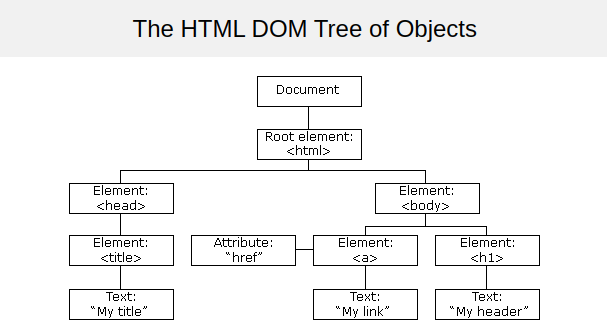
\includegraphics[scale=0.7]{Picture/mobile/dom_tree.png}
		\caption{DOM Tree of Objects}
		\label{fig:dom_tree}
	\end{figure}
}
\subsubsection{Virtual Document Object Model}
\par{
	The virtual DOM (VDOM) is a programming concept where an ideal, or “virtual”, representation of a UI is kept in memory and synced with the “real” DOM by a library such as ReactDOM. This process is called reconciliation.

	This approach enables the declarative API of React: You tell React what state you want the UI to be in, and it makes sure the DOM matches that state. This abstracts out the attribute manipulation, event handling, and manual DOM updating that you would otherwise have to use to build your app.

	Since “virtual DOM” is more of a pattern than a specific technology, people sometimes say it to mean different things. In React world, the term “virtual DOM” is usually associated with React elements since they are the objects representing the user interface. React, however, also uses internal objects called “fibers” to hold additional information about the component tree. They may also be considered a part of “virtual DOM” implementation in React.

}
\subsubsection{Reconciliation}
\par{
	When a component’s props or state change, React decides whether an actual DOM update is necessary by comparing the newly returned element with the previously rendered one. When they are not equal, React will update the DOM. This process is called “reconciliation”.
}
\subsubsection{One-way data flow}
\par{
	Neither parent nor child components can know if a certain component is stateful or stateless, and they shouldn’t care whether it is defined as a function or a class.

	This is why state is often called local or encapsulated. It is not accessible to any component other than the one that owns and sets it.

	A component may choose to pass its state down as props to its child components:

	\begin{figure}[!ht]
		\centering
		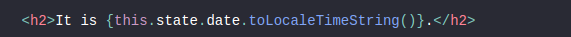
\includegraphics[scale=0.7]{Picture/mobile/data_flow_1.png}
		\label{fig:data_flow_1}
	\end{figure}

	This also works for user-defined components:

	\begin{figure}[!ht]
		\centering
		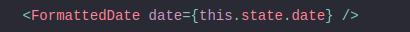
\includegraphics[scale=0.7]{Picture/mobile/data_flow_2.png}
		\label{fig:data_flow_2}
	\end{figure}

	The FormattedDate component would receive the date in its props and wouldn’t know whether it came from the Clock’s state, from the Clock’s props, or was typed by hand:

	\begin{figure}[!ht]
		\centering
		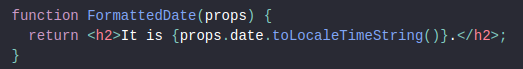
\includegraphics[scale=0.7]{Picture/mobile/data_flow_3.png}
		\label{fig:data_flow_2}
	\end{figure}

	This is commonly called a “top-down” or “unidirectional” data flow. Any state is always owned by some specific component, and any data or UI derived from that state can only affect components “below” them in the tree.

	If you imagine a component tree as a waterfall of props, each component’s state is like an additional water source that joins it at an arbitrary point but also flows down.


}
\subsubsection{Component and props}
\par{
	Components let you split the UI into independent, reusable pieces, and think about each piece in isolation.
	Conceptually, components are like JavaScript functions. They accept arbitrary inputs (called “props”) and return React elements describing what should appear on the screen.
	}
\subsection{React native}
\subsubsection{Overview}
React native is an open-source javascript mobile application 
framework which easily let developers create fully native 
mobile applications. Allow Taking advantages of powerful React core, 
React Native has been proving its performance as well as scalable 
feature on multi-platform application. In this Section, we will 
discuss about core concepts of React Native and explain how React 
Native's performance is optimize and responsive in multi-platform versions. 
Last but not least, We present how we construct data management in React Native.\\
\subsubsection{Architecture}
React Native is a compose of four sections which are React section, Javascript compiler, bridge section, native section. In general, there are two realms, javascript one and native one, which asynchronously communicate back and forth through a bridge. As specified in \ref{fig:RN-architecture}.\\
	
\begin{figure}[!h]
		\centering
		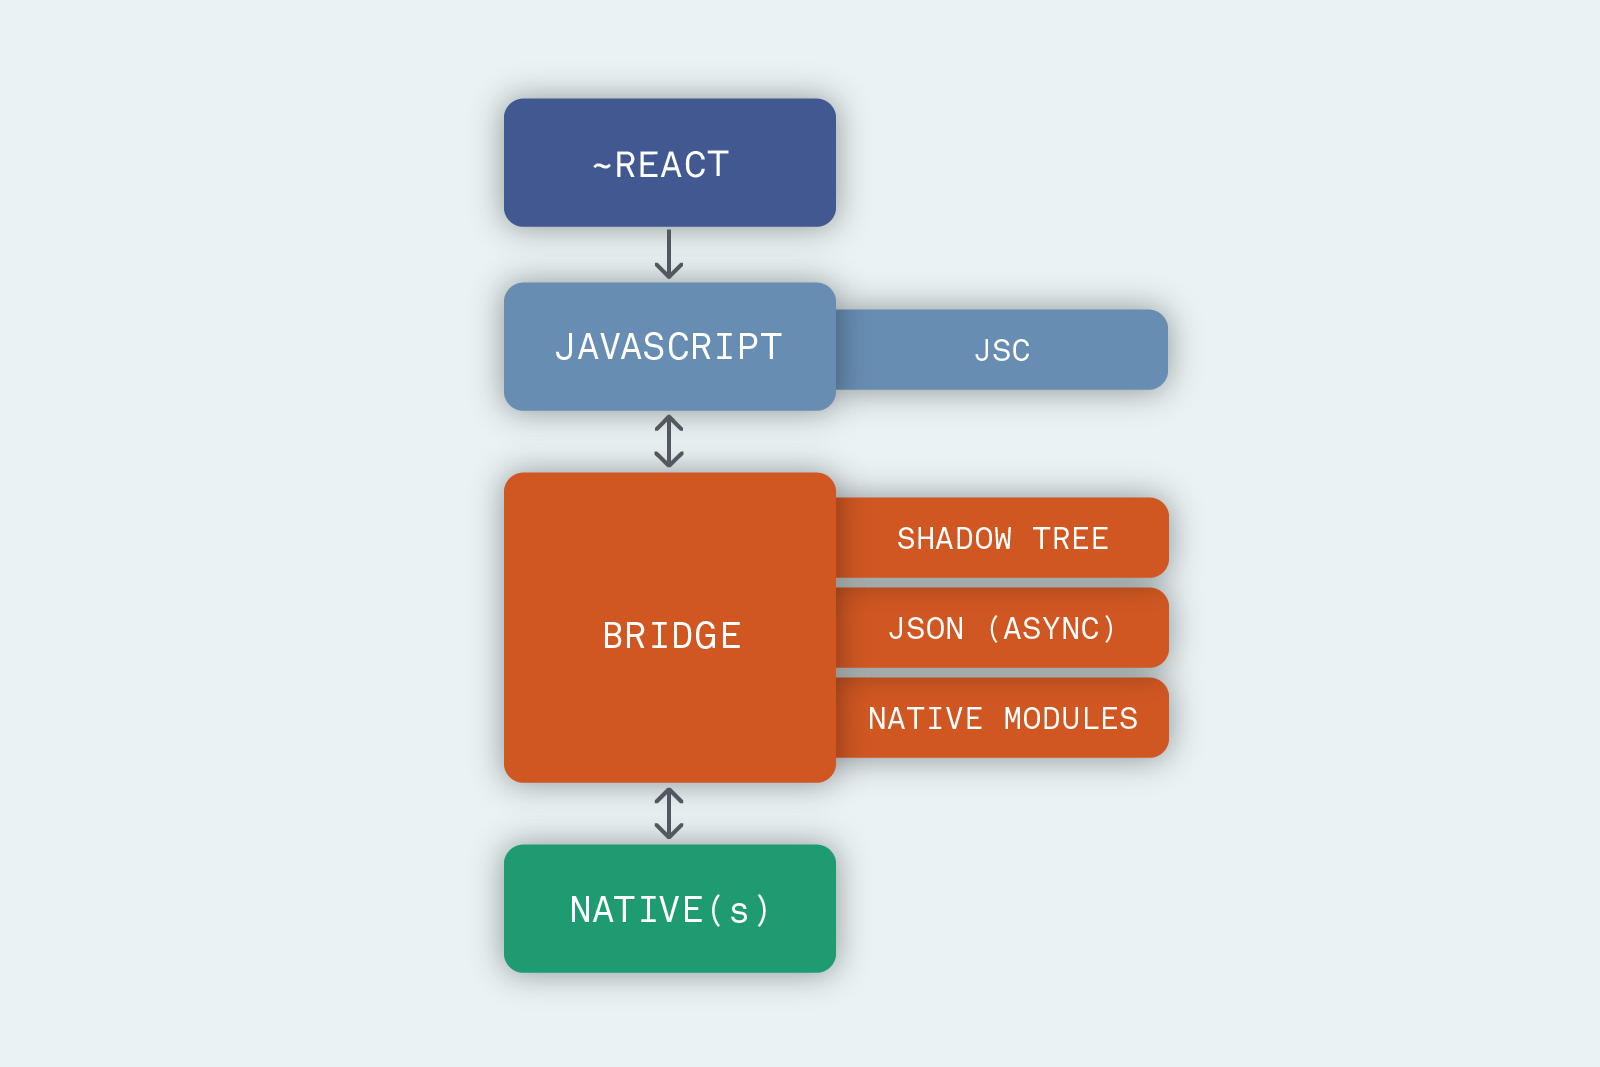
\includegraphics[scale=0.4]{Picture/mobile/RN-architecture.png}
		\caption{React native's general architecture}
	\label{fig:RN-architecture}
\end{figure}
	
	
When it comes to communication between multiple platforms (multi-services communication, different technologies), it is popular to use interoperable languages, such as JSON or XML in order to deliver data between 2-separated platforms, so does React Native. It uses JSON as a standard simple lightweight medium to transfer information between Javascript side and native side which are two different environments as well. Figure below illustrate the process \ref{fig:RN-communication-JSON}\\
Asynchronous communication between two realm in React Native benefit performance stuff. Firstly, because of not locking execution of the program, React Native are easily achieve ~60fps which make the application run smoothly on most of the case. Secondly, It can easily integrate other independent components latter or in other words it can open to other rendering system (Window OS, desktop, etc..). Another reason why React Native choose JSON as an interoperable languages is that it is ubiquitous and universal, which are built in and accepted most of technologies as well as different platforms.\\

\begin{figure}[!h]
		\centering
		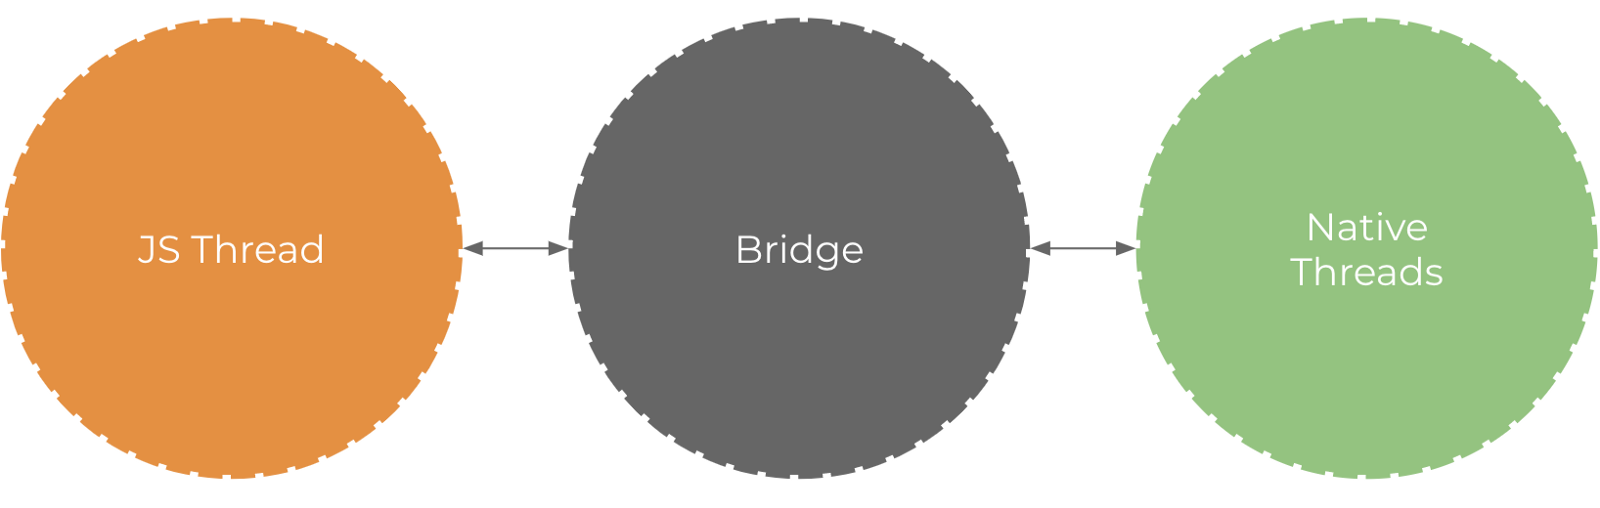
\includegraphics[scale=0.2]{Picture/mobile/communication-bridge.png}
		\caption{JS side communicates with the native side through the bridge}
	\label{fig:RN-communication-JSON}
\end{figure}
	

\subsubsubsection{React Core in React Native}

As mention in previous section~\ref{React-core}, React Native makes use of the power of React where Virtual DOM bring best performance to the application. Like React JS on web development, React Native also maintains a virtual DOM which define initial layout and make use of the diff algorithm to optimize the heavy UI-rendering process whenever happening changes of state in the application.\\ 
	
\begin{figure}[!h]
   	\centering
    	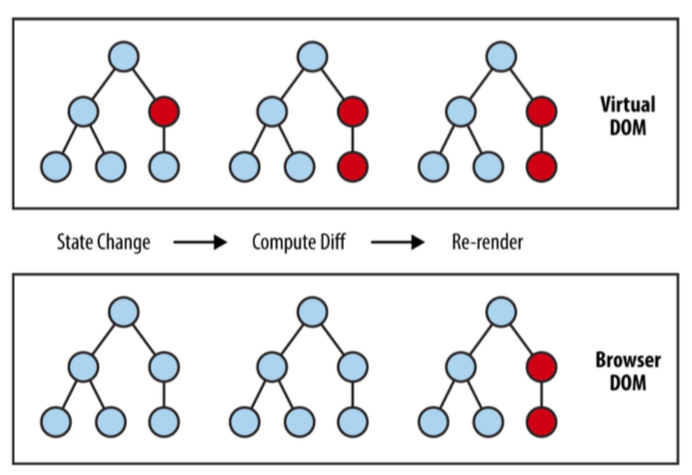
\includegraphics[scale=0.4]{Picture/mobile/RN-virtualDOM.png}
       	\caption{React's virtual DOM}
	\label{fig:RN-virtualDOM}
\end{figure}
	
JSX looks like HTML and style in React Native are css-like language has turned this technology into easy to learn and write framework.\\
	
\begin{figure}[!h]
   	\centering
    	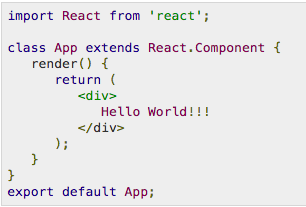
\includegraphics[scale=0.7]{Picture/mobile/RN-code.png}
        	\caption{React Native's coding style}
	\label{fig:RN-code}
\end{figure}
	
\subsubsubsection{Javascript Virtual Machine(JVM)}


Javascript virtual machine is a program or interpreter which executes Javascript code. React Native uses JavascriptCore to run code and most of the time, developers implement application by Javascript which will then be executed and asynchronously communicate with native code through the bridge.

\begin{itemize}
\item In case of iOS, JavascriptCore was intrinsically install in iOS platform which is the Javascript engine to power Safari and React Native uses available JavascriptCore provided by iOS platform so that it hand React Native the ability to evaluate JavaScript programs from within Swift, Objective-C, and C-based apps. Thus, physical event like touch, swipe, ... are able to transfer signals back to javascript logic to handle and execute
\item In case Android, unfortunately, JavascriptCore has been not installing in Android. React Native has to bundle JavascriptCore along with application, which increase the app's size. 
\item In web browser, because React Native use JavascriptCore so it can easily take advantages of Chrome debugging tool such as network request, console logs, etc... 
\end{itemize}

\subsubsubsection{React Native Brigde}
React Native bridge is built in C/C++ thus it can be run on multiple platforms, OS, etc... Making use of this power, React Native asynchronous sends information into the bridge through message queue. The picture \ref{fig:RN-process-communication} illustrate clearly about this process.
	
\begin{figure}[!h]
   	\centering
    	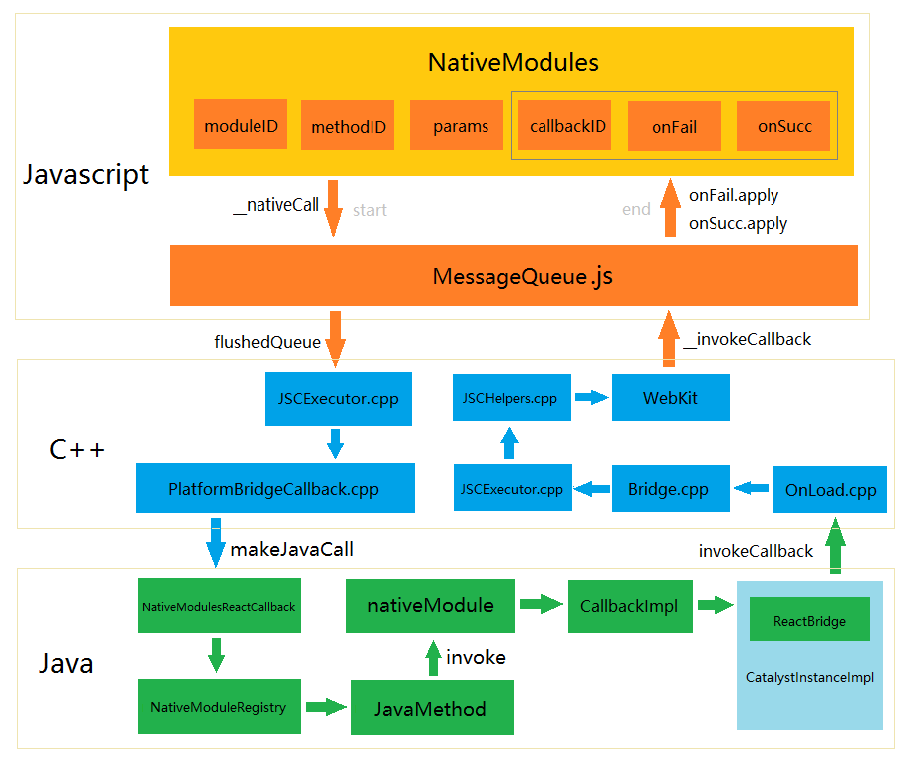
\includegraphics[scale=0.5]{Picture/mobile/RN-bridge.png}
     	\caption{The process of asynchronous communicating information between JS side and native side}
	\label{fig:RN-process-communication}
\end{figure}
	
As we can see, the Javascript code first create data and send to message queue which is still run on JS environment. After that, it will trigger C++ modules with defined protocol as parameter.

When the bridge is activated by message queue, it carries to call APIs of native modules with appropriate cases:

\begin{itemize}
\item In iOS, Obj-C is an extension of C language, so the bridge can natively communicate iOS APIs which is implemented by Obj-C. Hence, trigger actions, events back end forth are fast and natural
\item In Android, the bridge interact native modules through Java Native Interface. 
\end{itemize}

When React Native want to render some View from logic Javascript code, it sends data to the bridge through JSON-formatting protocol which is shown in the below image \ref{fig:RN-json-message}. To be more specific about this protocol, React Native has created a set of UI kit with correspond modules' identifies in native code and whenever it need render some layout on screen from Javascript, it passes module's identifier and some extra information about that module such as styling, native UI events, etc... then it will be executed in native environments and display suitable UI components with regarding module's identifier.
	
\begin{figure}[!h]
   	\centering
    	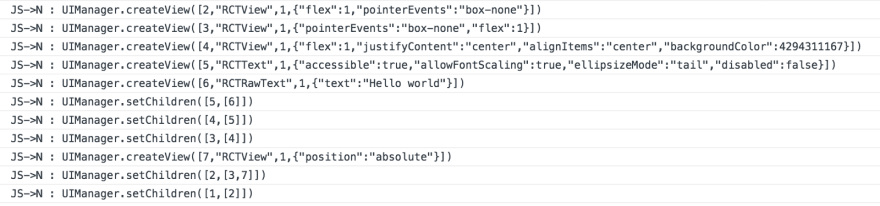
\includegraphics[scale=0.4]{Picture/mobile/RN-json-message.png}
    	\caption{JSON-formatting protocol}
	\label{fig:RN-json-message}
\end{figure}
	
To summarize, the bridge is basically an auxiliary to call forth native modules and send information, UI events back to Javascript thread. 

\subsubsubsection{Threading Model}
To be able to run cross-platform application, React Native basically need three vital modules which are JS thread, native module thread and native thread. These threads are spawned when React Native's app is first launched. Let's discuss more detail about these threads and how they work. 

\begin{figure}[!h]
   	\centering
    	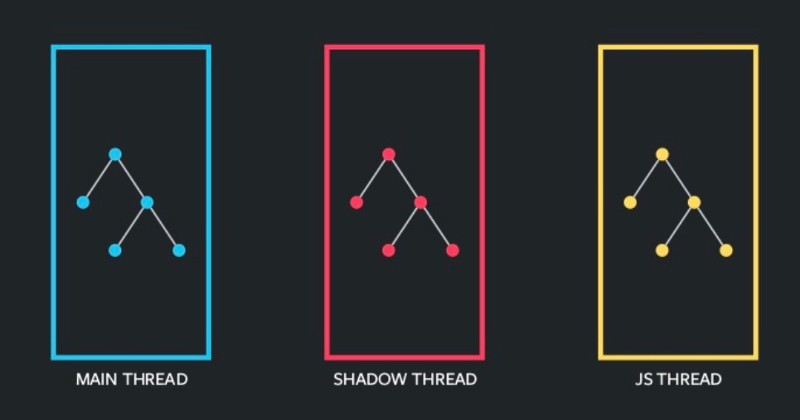
\includegraphics[scale=0.4]{Picture/mobile/RN-thread.jpeg}
    	\caption{React native threads}
	\label{fig:RN-threads}
\end{figure}

\begin{itemize}
\item \textbf{Native thread} (main thread) is the thread which lie in native platform and mainly take the responsibilities of rendering UI on native mobile screen as well as receiving physical-interacting events such as "press", "hold", "shake", etc. To be more specific, on native side, before rendering on the screen, it needs to calculate the layouts of the application in shadow thread. Besides, Intuitively, native thread listens the incoming events from users or internal platform events and these events will be turned into JSON-formatting packages and asynchronous transferred back to JS thread where the logic of the mobile's app is executed.
\item \textbf{Shadow thread} is an engine which calculate the position of views, how it should be positioned or colored and then these information will be sent back to main thread to proceed to render the view
\item	\textbf{Javascript thread} is where all logic execution happen. This thread is responsible for processing business logic, receiving all information from native thread. Theoretically, Javascript code is executed on single thread. Thus, some heavy-calculating tasks will cause slow in performance like image processing, face recognizing, etc...or animation. 
\item \textbf{Native module thread} is the thread which are spawned from React Native to handle some custom modules. Custom modules are used to access native platform's APIs which are not provided by React Native and also custom modules which are written by native code significantly increase performance. Practically, most heavy-calculating tasks are written in this modules to defer "bottle neck" problem in JS thread which is single thread. 
\end{itemize}

Now, we discuss about the interaction between these threads, how it effectively works in different platforms. Let's visualize the process by taking a look in the picture \ref{fig:RN-threads-visualization}

\begin{enumerate}
\item At the beginning, the application will launch main thread (native thread) and the main thread will load JS bundles (JS bundles is all the React Native code is put into a single file by using Webpack to make it easily load instead of loading multiple files) 
\item When the JS bundles are successfully loaded, and start JS thread to execute JS code. From now, JS thread generates new Virtual DOM and send it into shadow thread to calculate layout
\item The main thread is responsible for rendering the view on screens. Hence, shadow thread sends generated layout to main thread in order to render UI.
\item After completely rendering UI in main threads, it will send some information back to JS thread to announce that it has successfully rendered the View and JS thread can trigger correspond componentDidMount function as mention in \ref{React}
\item When custom modules are called from JS, the information will be sent through the React Native's bridge and then be executed on native custom modules as visualizing in the below picture
\end{enumerate}

\begin{figure}[!h]
   	\centering
    	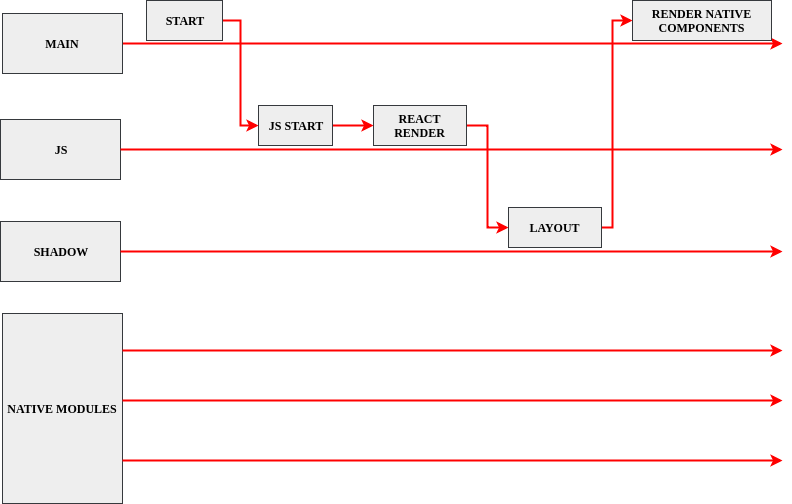
\includegraphics[scale=0.4]{Picture/mobile/RN-threads.png}
    	\caption{Visualize threads in React Native}
	\label{fig:RN-threads-visualization}
\end{figure}

\subsubsection{React Native's future upgrade}
In the previous section, we discuss the architecture of React Native and how it can smoothly run on different platforms (iOS and Android). However, there are still have many long-standing issues of cross-platform application. Announce in 2018, The Facebook's team has massively put many efforts to re-architecture React Native to make it run more effective and smoother by reducing some redundant stages or add some new components to tackle cross-platform problems. 

As illustrating in the figure \ref{fig:RN-new-architecture} and comparing to the current architecture \ref{fig:RN-architecture}, Facebook' team divided the bridge into two main sections, Fabric and Turbo modules. 
\begin{itemize}
\item Fabric aims to remove the long process of rendering UI, which are currently React -> Native -> Shadow Tree -> Native UI, and new upgrade will directly generate shadow tree from C++. Hence, to rendering UI, it does not have to call native thread, then call shadow thread and then call native thread to render, it will hugely improve the responsiveness of performance. 
\item Normally, many native modules used by Javascript code is intrinsically initialized when the application is launched because of the unawareness between two side (JS one and native one), this make the process of launching the application long. With new upgrade, the Turbo will initialize only when it needs by JS thread.
\end{itemize}

Furthermore, we can notice that there is a considerable amount of code removed in native section which makes the app's size smaller 
\begin{figure}[!h]
   	\centering
    	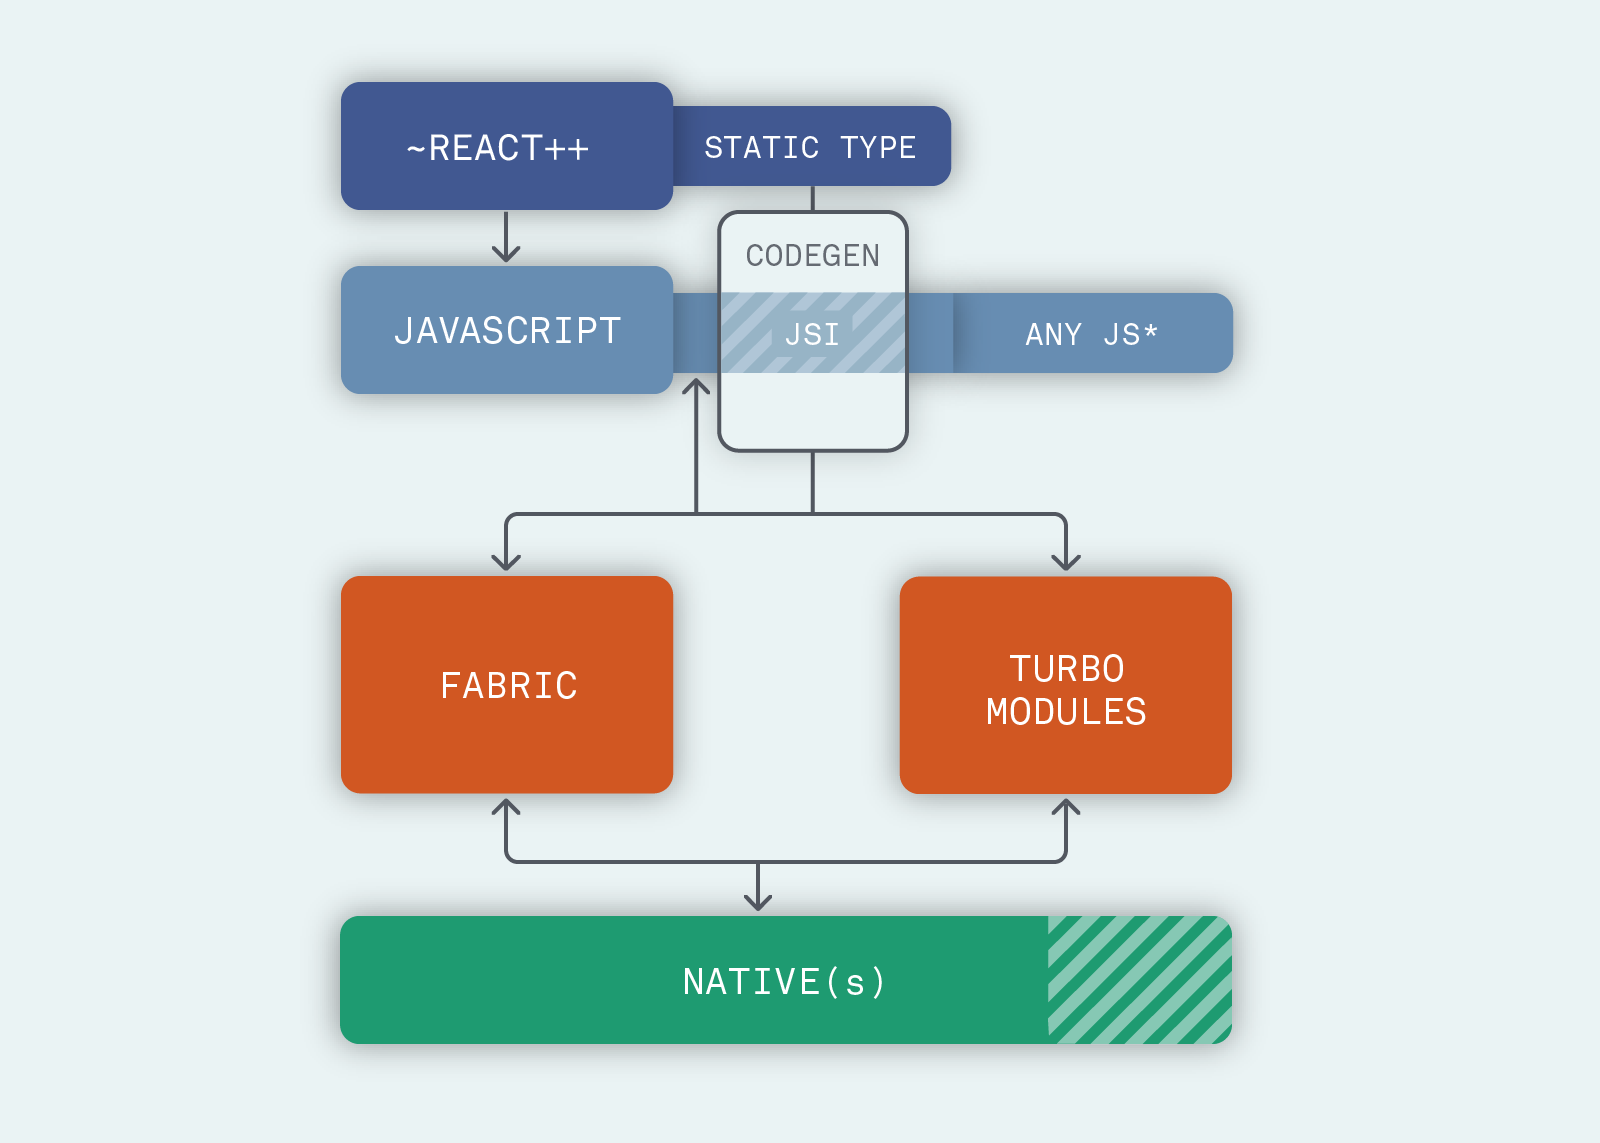
\includegraphics[scale=0.4]{Picture/mobile/RN-new-architecture.png}
    	\caption{New proposed architecture of React Native}
	\label{fig:RN-new-architecture}
\end{figure}

\section{Server Application}
\subsection{Overall architecture}
\subsubsection{Threading model}
\subsubsubsection{Multi-threaded server}
Traditionally, typical web servers handle multiple requests by threading. Each incoming request spawns a separate thread (or use a thread from a thread pool to improve performance \cite{thread_pool}), thus allowing the server to serve multiple requests concurrently. However, the drawbacks to this approach are more apparent as the number of requests grow. First of all, computer resources is limited, so performance starts to degrade significantly if the system run out of resources. Secondly, in a multi-threaded server, if there is a problem in synchronization, all the threads will crash, effectively rendering the server unresponsive.

\begin{figure}[!h]
	\centering
	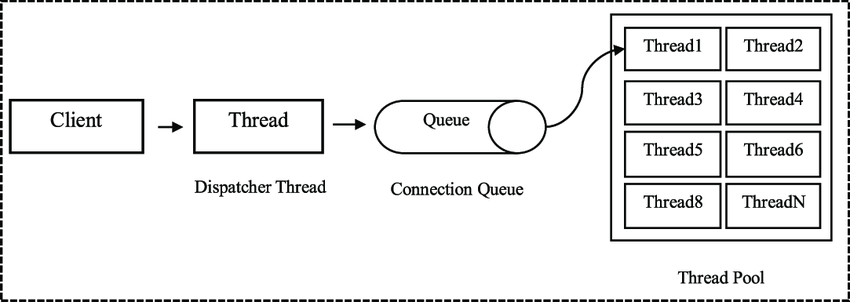
\includegraphics[scale=0.4]{Picture/server/multithreaded-server-architecture.png}
	\caption{A thread pool based server architecture}
\label{fig:multithreaded-server}
\end{figure}

Some of the web servers utilizing this architecture are Apache HTTP Server \cite{apache} and Microsoft IIS \cite{iis}.

\subsubsubsection{Event-driven server}
In an event-driven server, when a request comes in, the event is dispatched and a handler will pick it up. Typically, there is an event loop, which will go over these events and pick it up to process if it is free.

In a web server, this means that a lot of requests can be served at the same time with just a single thread, without the need to increase amount of hardware, reducing costs and allowing for horizontal scaling \cite{horizontal_scaling} - adding more nodes to a system, instead of adding resources to a single node.

The main drawback to this approach is that, if the request is computationally expensive, it will block other processes, or take too long to process. However, most web requests only involve IO operations (like IO fetching), which will be handled by the OS in (e.g. by utilizing a thread pool), thus are very suitable to this architecture.

\begin{figure}[!h]
	\centering
	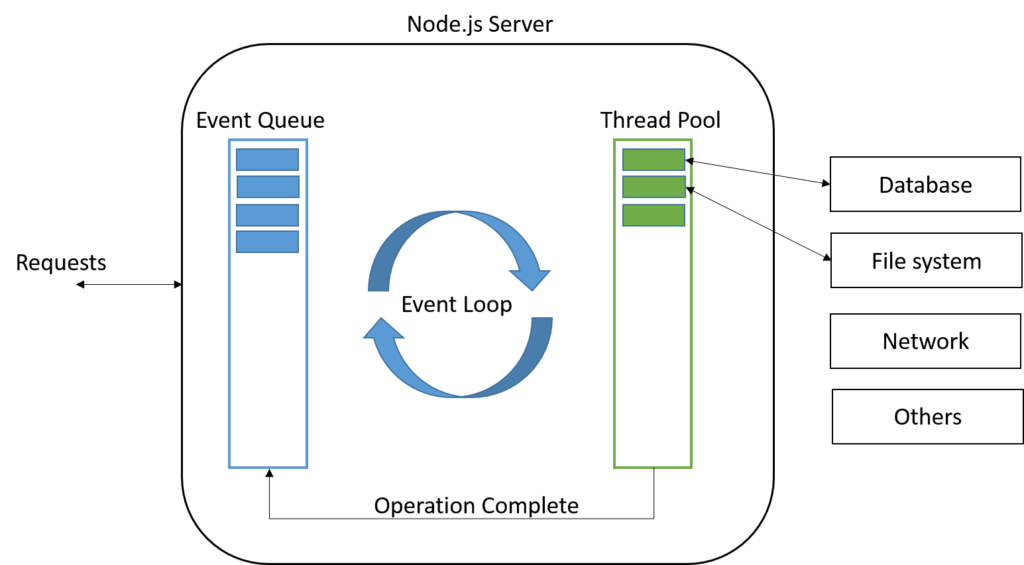
\includegraphics[scale=0.4]{Picture/server/event-loop-server.png}
	\caption{A server utilizing event loop architecture}
\label{fig:event-loop-server}
\end{figure}

Some of the web servers utilizing this architecture are Nginx \cite{nginx} and Node.js \cite{nodejs}.

\subsubsection{Node.js}
Node.js was written initially by Ryan Dahl, and first presented at JSConf EU 2009 \cite{jsconf}, addressing issues that are apparent in some of the most popular web servers of the time (e.g. Apache HTTP Server) in handling multiple concurrent requests (up to 10,000 requests \cite{c10k}).

Node.js combined Google's V8 JavaScript engine, an event loop, and a low-level I/O API. \cite{nodejs_structure}

Node.js brings event-driven programming to web servers, enabling development of fast web servers in JavaScript \cite{nodejs_structure}. Developers can create scalable servers without using threading, by using a simplified model of event-driven programming that uses callbacks to signal the completion of a task. Node.js connects the ease of a scripting language (JavaScript) with the power of Unix network programming. \cite{nodejs_structure}

\begin{figure}[!h]
	\centering
	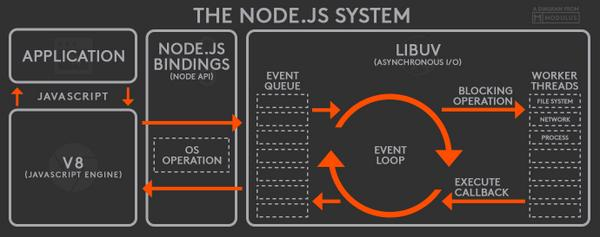
\includegraphics[scale=0.6]{Picture/server/node.jpg}
	\caption{Architecture of Node.js}
\label{fig:node}
\end{figure}

Therefore, for our project, we choose Node.js as the architecture behind our web server, due to the advantages stated above, as well as the amount of community resources available for it. With Node.js, we are able to create a high-performance and low-cost web server, with support for the latest technologies.

\subsection{Architecture}
With Node.js as the runtime, we then rely on a web framework to provide necessary features to accelerate development process. We settle on a framework called Nest.js for the following reasons:
\begin{itemize}
\item Modular architecture, with the concept of pluggable modules for easy integration, maintenance and testing.
\item Provides many modules out of the box, with extensive testing, allowing faster development.
\item Utilizing Dependency Injection, achieving Separation of Concerns of construction and use of objects, which promotes code reusablilty and readability.
\item Supports TypeScript, a typed superset of JavaScript \cite{typescript}, which aims to reduce common problem with JavaScript, namely loosely type checking and silent runtime errors, which can be very difficult to diagnose.
\end{itemize}

\subsubsection{Model-View-Controller}
Our application follows the Model-View-Controller (MVC) pattern. This pattern is used to separate program logic into three connected components:
\begin{itemize}
\item \textbf{Model}: The central component of the pattern. It is the application's dynamic data structure, independent of the user interface. It directly manages the data, logic and rules of the application. \cite{mvc_smalltalk}
\item \textbf{View}: Any representation of information such as a chart, diagram or table. Multiple views of the same information are possible, such as a bar chart for management and a tabular view for accountants.
\item \textbf{Controller}: Accepts input and converts it to commands for the model or view \cite{mvc_controller}
\end{itemize}
In addition to dividing the application, the MVC pattern also defines the relationship between them: \cite{mvc_relationship}
\begin{itemize}
\item The model is responsible for managing the data of the application. It receives user input from the controller.
\item The view means presentation of the model in a particular format.
\item The controller responds to the user input and performs interactions on the data model objects. The controller receives the input, optionally validates it and then passes the input to the model.
\end{itemize}

\begin{figure}[!h]
	\centering
	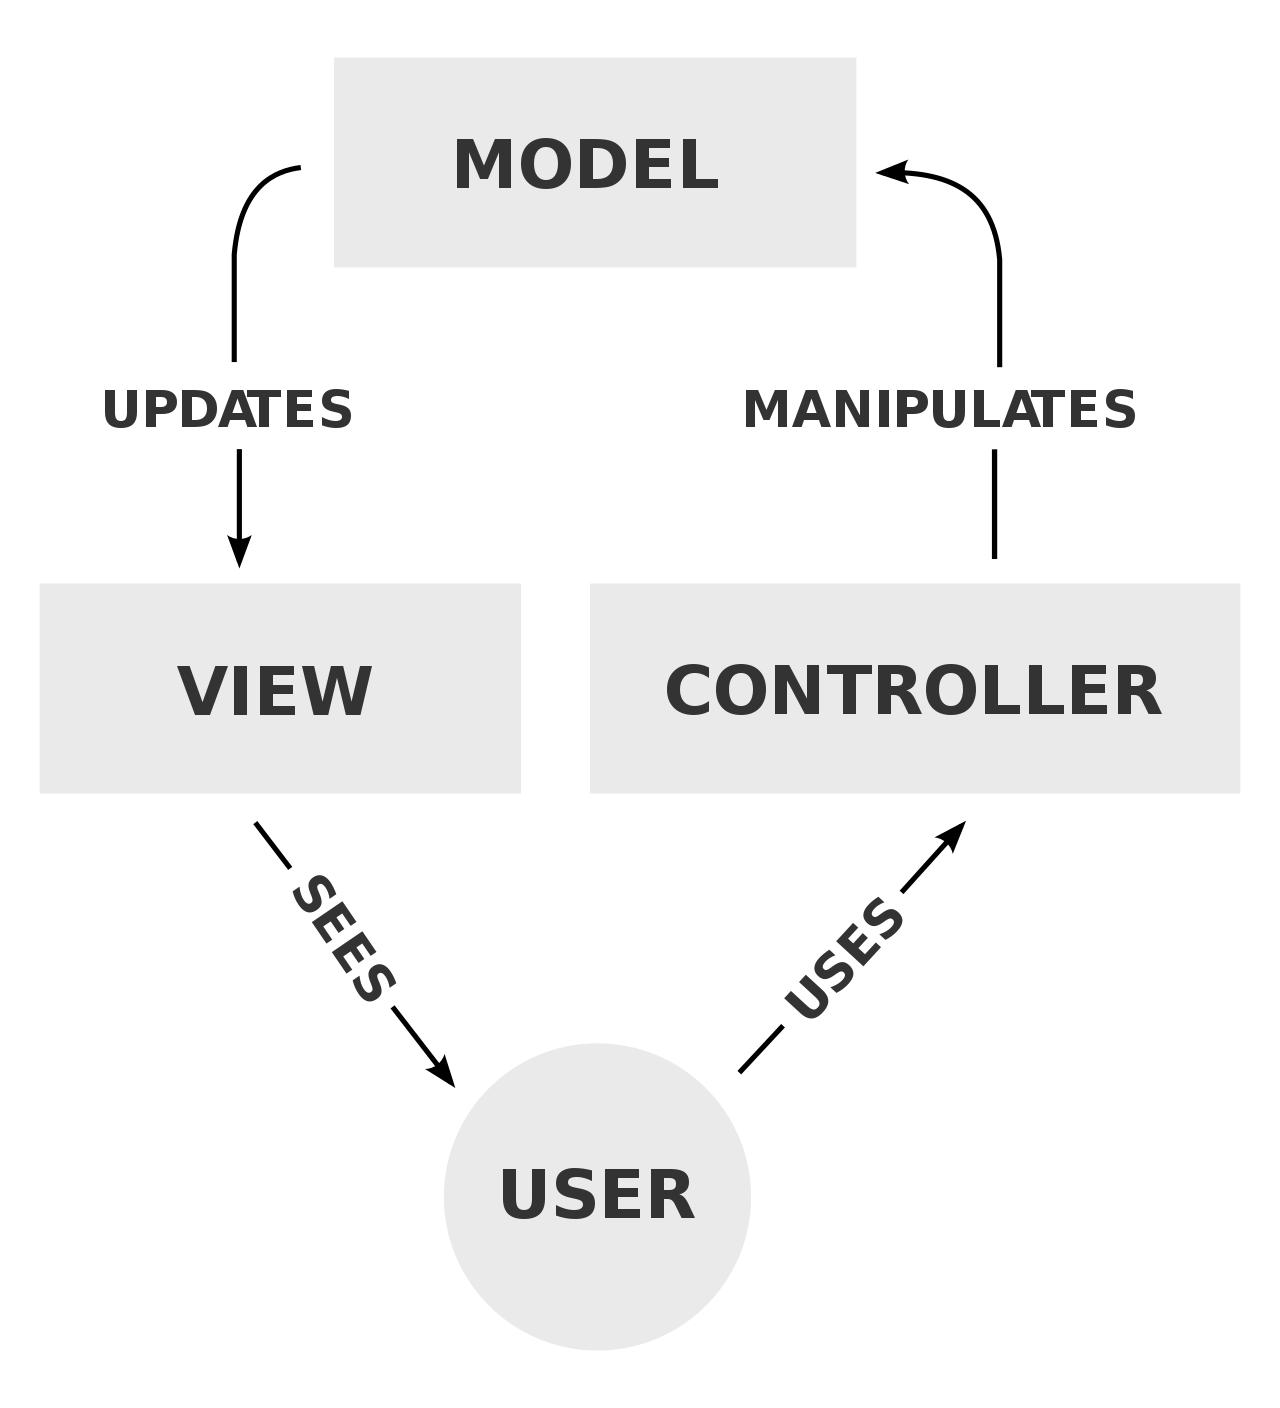
\includegraphics[scale=0.15]{Picture/server/mvc.png}
	\caption{Diagram of interactions within the MVC pattern}
\label{fig:mvc}
\end{figure}

In our application, the View layer is handled the mobile application, which  displays the data provided by the model when it dispatches commands via the controller. Moreover, our application extends the MVC model with the addition of:
\begin{itemize}
\item \textbf{Services}, which aim to move the logic out of the controller, allowing better code reuse and keep the controllers slim, and achieve better separation of concerns, where the controllers only manage the data flow.
\item \textbf{Repositories}, which is an abstraction layer above the model, allowing for more simple data access, without the need to use platform-specific features of the persistence layer underneath, thus allowing the code to be more portable, and less tied to the underlying database architecture underneath.
\end{itemize}

\subsubsection{Dependency Injection}
Dependency Injection is a technique whereby one object supplies the dependencies of another object. A "dependency" is an object that can be used, for example as a service. The intent behind dependency injection is to achieve Separation of Concerns of construction and use of objects. This can increase readability and code reuse.

Dependency injection separates the creation of a client's dependencies from the client's behavior, which allows program designs to be loosely coupled and to follow the dependency inversion and single responsibility principles.

Dependency injection involves 4 roles:
\begin{itemize}
\item the \textbf{service} object(s) to be used
\item the \textbf{client} object that is depending on the service(s) it uses
\item the \textbf{interfaces} that define how the client may use the services
\item the \textbf{injector}, which is responsible for constructing the services and injecting them into the client
\end{itemize}
There are many advantages to this approach:
\begin{itemize}
\item Isolates the client from changes of other services, thus promoting reusability, testability and maintainability
\item Reduces coupling between a component and its dependencies
\item Allows concurrent development of different components. As long as the interfaces are defined, components can be developed independently of each other.
\end{itemize}

\begin{figure}[!h]
	\centering
	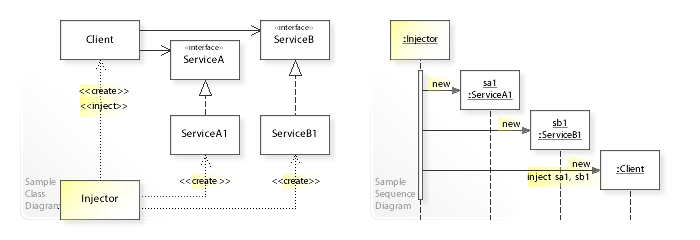
\includegraphics[scale=0.55]{Picture/server/di.jpg}
	\caption{A sample UML class and sequence diagram for the Dependency Injection design pattern. }
\label{fig:di}
\end{figure}

\subsubsection{Microservices Architecture (MSA)}
Microservices are a software development technique —a variant of the service-oriented architecture (SOA) structural style— that arranges an application as a collection of loosely coupled services. \cite{microservices}

\begin{figure}[!h]
	\centering
	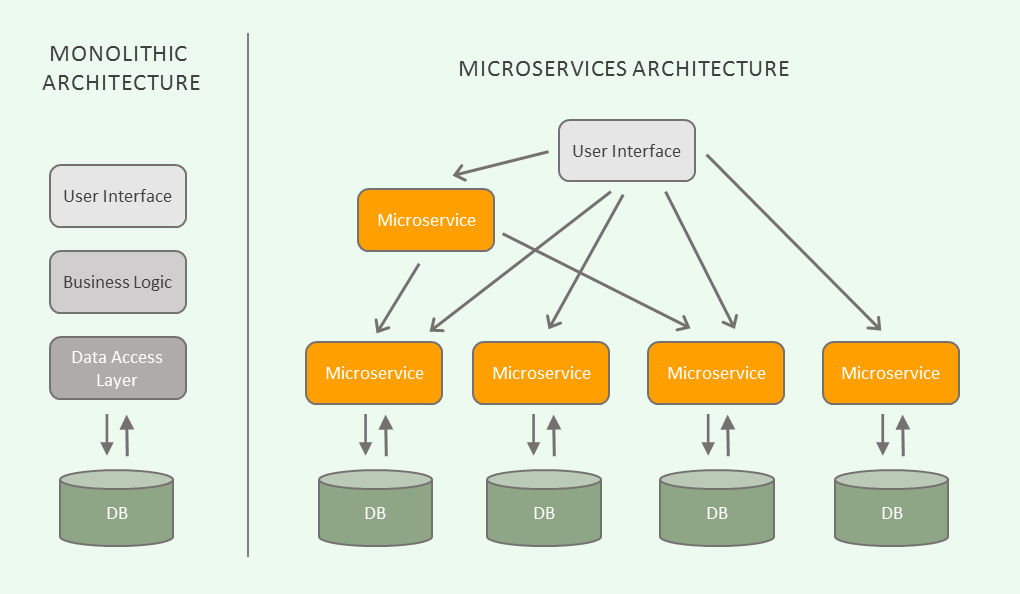
\includegraphics[scale=0.3]{Picture/server/microservices.png}
	\caption{Comparison between microservices and monolithic architectures.}
\label{fig:msa}
\end{figure}

Some characteristics of microservices include:
\begin{itemize}
\item Services in a microservice architecture (MSA) are often processes that communicate over a network to fulfill a goal using technology-agnostic protocols such as HTTP. \cite{microservices_newman}
\item Services in a microservice architecture are independently deployable. \cite{microservices_ieee}
\item Services can be implemented using different languages, hardware and software components, depending on what fits best. \cite{microservices_ieee}
\end{itemize}

This approach brings many benefits:
\begin{itemize}
\item \textbf{Modularity}: This makes the application easier to understand, develop, test, and become more resilient to architecture erosion \cite{microservices_ieee}, compared to traditional monolithic approach.
\item \textbf{Scalability}: Services are independent of each other, thus can be maintained, monitored and scale independently.
\end{itemize}

\section{Blockchain}
